\input ../SlidePreamble
\input ../preamble


\begin{document}

{\Huge

  \centerline{\bf TTIC 31230, Fundamentals of Deep Learning}
  \bigskip
  \centerline{David McAllester, Winter 2019}
  \vfill
  \centerline{Rate-Distortion Autoencoders (RDAs)}
  \vfill
  \centerline{Noisy Channel RDAs}
  \vfill
  \centerline{Gaussian Variational Autoencoders (Gaussian VAEs)}

\slide{Rate-Distortion Autoencoders}

Given a continuous signal $y$ we can compress it into a (discrete) bit string $\tilde{z}_\Phi(y)$.

\vfill
We let $y_\Phi(\tilde{z}_\Phi(y))$ be the decompression of $\tilde{z}_\Phi(y)$.

\vfill
We can then define a rate-distortion loss.

{\color{red} $${\cal L}(\Phi) = E_{y \sim \mathrm{Pop}}\;|\tilde{z}_\Phi(y)| + \lambda \mathrm{Dist}(y,y_\Phi(\tilde{z}_\Phi(y)))$$}

\slide{Common Distortion Functions}

$$\Phi^* = \argmin_\Phi\;E_{y \sim \mathrm{Pop}}\;|\tilde{z}_\Phi(y)| + \lambda \mathrm{Dist}(y,y_\Phi(y))$$

\vfill
It is common to take

$$\mathrm{Dist}(y,y') = ||y-y'||^2 \hspace{4em}(L_2)$$

\vfill
or

$$\mathrm{Dist}(y,y') = ||y-y'||_1 \hspace{4em} (L_1)$$

\slide{A Case Study in Image Compression}

{\bf End-to-End Optimized Image Compression, Balle, Laparra, Simoncelli, ICLR 2017.}


\vfill
$${\color{red}y \hspace{5em}  \tilde{z}_\Psi(y) \hspace{4em} \tilde{z} \hspace{6em} y'_\Phi(\tilde{z}) \hspace{4em}||y - y'||^2}$$
\centerline{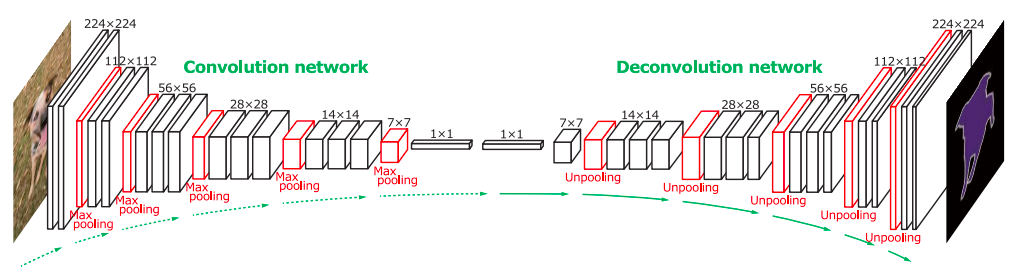
\includegraphics[width=9in]{../images/Deconv}}

\anaslide{JPEG at 4283 bytes or .121 bits per pixel}

\bigskip
\centerline{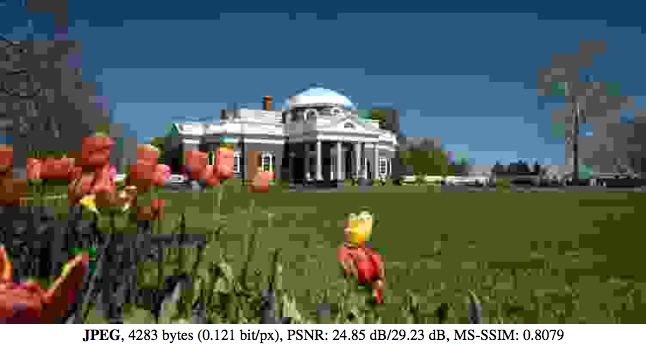
\includegraphics[height=5in]{../images/RateDist2}}

\anaslide{JPEG 2000 at 4004 bytes or .113 bits per pixel}

\bigskip
\centerline{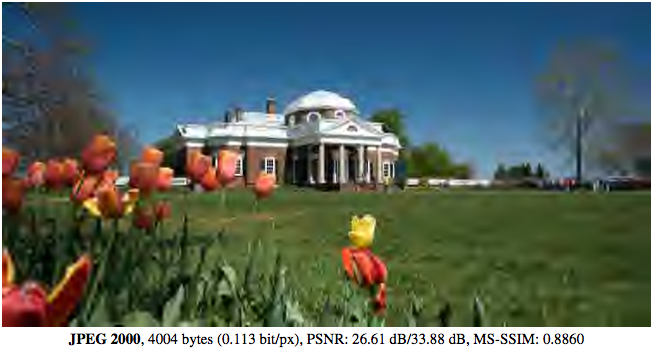
\includegraphics[height= 5in]{../images/RateDist3}}

\anaslide{Deep Autoencoder at 3986 bytes or .113 bits per pixel}

\bigskip
\centerline{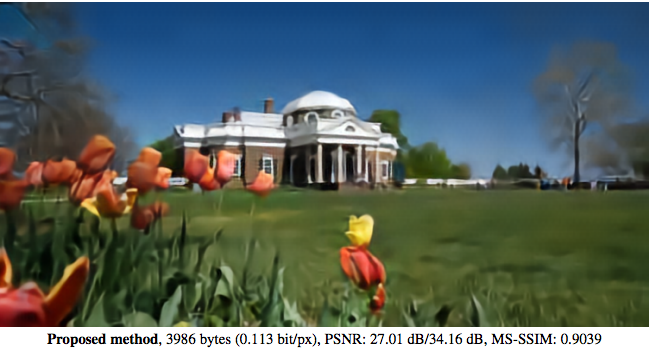
\includegraphics[height = 5in]{../images/RateDist4}}

\slide{A CNN Encoder}

A three layer CNN is used as an encoder.

\vfill
We let $z_\Phi(y)$ be the final layer of this CNN.

\vfill
Each continuous value in the final layer $z_\Phi(y)$ is then rounded to a (small) integer giving a discrete encoding $\tilde{z}(y)$.

\slide{Rate-Distortion Autoencoders}

$$\Phi^* = \argmin_\Phi \;E_{y \sim \pop}\;|\tilde{z}_\Phi(y)| + \lambda \mathrm{Dist}(y,y_\Phi(\tilde{z}_\Phi(y)))$$

\vfill
Oops: Because of rounding, $\tilde{z}_\Phi(y)$ is discrete and the gradients are zero.

\vfill
We will train using a differentiable approximation.

\slide{A Noise Model of Rounding}

We can make distortion differentiable by modeling rounding as the addition of noise.

\begin{eqnarray*}
{\cal L}_{\mathrm{dist}}(\Phi) & = & E_{y \sim \mathrm{Pop}} \;\mathrm{Dist}(y,y_\Phi(\tilde{z}_\Phi(y))) \\
\\
& \approx & E_{y,\epsilon} \;\mathrm{Dist}(y,\;y_\Phi(z_\Phi(y) + \epsilon))
\end{eqnarray*}

\vfill
Here $\epsilon$ is a noise vector each component of which is drawn uniformly from $(-1/2,1/2)$.

\slide{Noise vs. Rounding}

\centerline{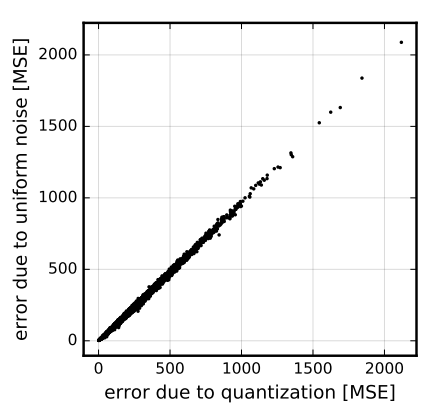
\includegraphics[height=5in]{../images/RateDist5}}


\slide{A Differentiable Approximation of Code Length}

\begin{eqnarray*}
{\cal L}_{\mathrm{rate}}(\Phi) & = & E_{y \sim \pop}\;|\tilde{z}_\Phi(y)| 
\end{eqnarray*}

\vfill
Recall that {\color{red} $\tilde{z}_\Phi(y)$} is a rounding of a continuous encoding {\color{red} $z_\Phi(y)$}.


\vfill
We approximate the code length after rounding using a differentiable function of the value before rounding.

\vfill
{\color{red} $$|{\color{red} \tilde{z}_\Phi(y)}| \approx \sum_i (\log_2 {\color{red} z_\Phi(y)[i]})^+$$}

This continuous value can be interpreted as a ``differential entropy''.

\slide{Differential Entropy vs. Discrete Entropy}

\bigskip
\centerline{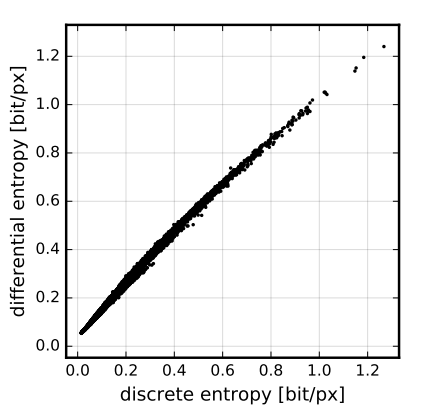
\includegraphics[height=5in]{../images/RateDist6}}


\slide{Details}

\vfill
The first layer is computed stride 4.

\vfill
The next two layers are computed stride 2.

\vfill
Final image dimension is reduced by a factor of 16 with 192 channels per pixel (192 channels is for color images).

\vfill
$$192 < 16 \times 16 \times 3 = 768$$

\vfill


\slide{Increasing Spatial Dimension in Decoding}

\centerline{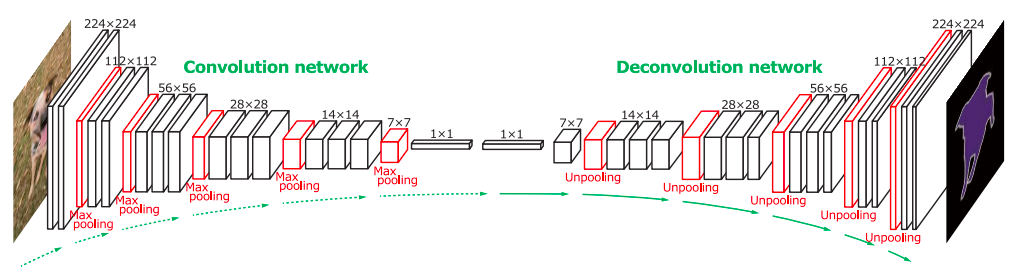
\includegraphics[width=9in]{../images/Deconv}}
\centerline{[Hyeonwoo Noh et al.]}

\vfill
In the ICLR 17 paper the deconvolution network has the shape as the input CNN but with independent parameters.

\slide{Increasing Spatial Dimension in Decoding}

Consider a stride 2 convolution
\begin{eqnarray*}
  L_{\ell+1}[x,y,j] & = & \sigma\left(\sum_{\Delta x,\Delta y,i}   W[\Delta x, \Delta y, i,j] L_\ell[2x + \Delta x, 2y + \Delta y, i]\right)
\end{eqnarray*}

\vfill
For deconvolution we use stride 1 with 4 times the features.
\begin{eqnarray*}
  L'_\ell[x,y,i] & = & \sigma\left(\sum_{\Delta x,\Delta y,j}   W[\Delta x, \Delta y, j,i] L'_{\ell+1}[x + \Delta x, y + \Delta y, j]\right)
\end{eqnarray*}

\vfill
The channels at each $L'_\ell[x,y]$ are divided among four higher resolution pixels.

\vfill
This is done by a simple reshaping of $L'_\ell[x,y,i]$.

\slide{Noisy-Channel RDAs (TZ)}

Consider the differentiable loss used in training.
{\color{red} $$\Phi^* = \argmin_\Phi \;E_{y \sim \pop}\;- \ln p(z_\Phi(y)) + \lambda E_\epsilon\; \mathrm{Dist}(y,y_\Phi(z_\Phi(y) + \epsilon))$$}

Intuitively, {\color{red} $- \ln p(z_\Phi(y))$} is a proxy for the number of bits used in the (intuitively rounded) encoding {\color{red} $z_\Phi(y) + \epsilon$}.

\vfill
By the channel capcacity theorem the number of bits that {\color{red} $z_\Phi(y) + \epsilon$} can carry about {\color{red} $y$}
is the mutual information between $y$ and $z_\Phi(y) + \epsilon$.

{\color{red} $$I(y,z_\Phi(y)+\epsilon)$$}

\slide{Noisy-Channel RDAs}

We now consider {\color{red} $p_\Phi(z|y)$} as a generalization of {\color{red} $z_\Phi(y) + \epsilon$}.

\vfill
The channel capacity theorem motivates

$${\color{red} p_\Phi(z) = E_{y \sim \pop}\;p_\Phi(z|y)}$$
$${\color{red} I(y,z)} = H(z) - H(z|y) = {\color{red} E_{y \sim \pop}\;KL(p_\Phi(z|y),p_\Phi(z))}$$


\vfill
{\huge
\begin{eqnarray*}
{\color{red} \Phi^*} & = & \argmin_\Phi \left(\;{\color{red} I(y,z)} + \;\lambda E_{y \sim \pop,z \sim p_\Phi(z|y)}\;\mathrm{Dist}(y,y_\Phi(z))\;\right) \\
\\
& = & {\color{red} \argmin_\Phi  E_{y \sim \pop}\;\left(\begin{array}{l}\;\;\;\;KL(p_\Phi(z|y),p_\Phi(z)) \\
\\
+ \lambda E_{z \sim p_\Phi(z|y)}\; \mathrm{Dist}(y,y_\Phi(z))\end{array}\right)}
\end{eqnarray*}
}

\slide{A Variational Upper Bound}

Unfortunately we cannot compute {\color{red} $p_\Phi(z) = E_{y \sim \pop}\;p_\Phi(z|y)$}.

\vfill
We now replace {\color{red} $p_\Phi(z)$} by a friendly (variational) model {\color{red} $p_\Psi(z)$}.

\begin{eqnarray*}
 & & I_\Phi(y,z) \\
 \\
 & = & E_{y \sim \pop}\; KL(p_\Phi(z|y),p_\Phi(z)) \\
\\
& = & E_{y,z\sim P_\Phi(z|y)}\; \left(\ln \frac{p_\Phi(z|y)}{{\color{red} p_\Psi(z)}} + \ln \frac{{\color{red} p_\Psi(z)}}{p_\Phi(z)}\right) \\
\\
& = & E_{y \sim \pop}\;KL(p_\Phi(z|y),p_\Psi(z)) + \left(E_{y \sim \pop,\;z\sim p_\Phi(z|y)}\;\ln \frac{p_\Psi(z)}{p_\Phi(z)}\right)
\end{eqnarray*}

\slide{A Variational Upper Bound}

\begin{eqnarray*}
 & & I(y,z) \\
 \\
 & = & E_{y \sim \pop}\;KL(p_\Phi(z|y),p_\Psi(z)) + \left(E_{\color{red} y \sim \pop,\;z\sim p_\Phi(z|y)}\;\ln \frac{p_\Psi(z)}{p_\Phi(z)}\right) \\
\\
& = & E_y\;KL(p_\Phi(z|y),p_\Psi(z)) + E_{\color{red} z\sim p_\Phi(z)}\;\ln \frac{p_\Psi(z)}{p_\Phi(z)} \\
\\
& = & E_y\;KL(p_\Phi(z|y),p_\Psi(z)) - KL(p_\Phi(z),p_\Psi(z)) \\
\\
& \leq & E_{y \sim \pop}\; KL(p_\Phi(z|y),p_\Psi(z))
\end{eqnarray*}


\slide{The Noisy-Channel RDA}

{\color{red} $$\Phi^*,\Psi^* = \argmin_{\Phi,\Psi}\;E_{y\sim \pop} \left(\begin{array}{l}\;\;\;\;KL(p_\Phi(z|y),p_\Psi(z)) \\
\\
+ \lambda \; E_{z\sim p_\Phi(z|y)}\;\mathrm{Dist}(y,\;y_\Phi(z))\end{array}\right)$$}


\slide{Gaussian Noisy-Channel RDA}

$$\Phi^*,\Psi^* = \argmin_{\Phi,\Psi}\;E_{y\sim \pop} \left(\begin{array}{l}\;\;\;\;KL(p_\Phi(z|y),p_\Psi(z)) \\
\\
+ \lambda \; E_{z\sim p_\Phi(z|y)}\;\mathrm{Dist}(y,\;y_\Phi(z))\end{array}\right)$$

{\color{red}
\begin{eqnarray*}
p_\Phi(z[i]\;|\;y) & = & {\cal N}(z_\Phi(y)[i],\sigma_\Phi(y)[i])) \\
\\
p_\Psi(z[i]) & = & {\cal N}(\mu_\Psi[i],\sigma_\Psi[i]) \\
\\
\mathrm{Dist}(y,y') & = & ||y-y'||^2
\end{eqnarray*}
}

\slide{Closed Form KL-Divergence}

\begin{eqnarray*}
& & KL(p_\Phi(z|y),p_\Psi(z)) \\
\\
\\
& = & \sum_i \;\frac{\sigma_\Phi(y)[i]^2 + (z_\Phi(y)[i]-\mu_\Psi[i])^2}{2 \sigma_\Psi[i]^2}
+ \ln\frac{\sigma_\Psi[i]}{\sigma_\Phi(y)[i]} - \frac{1}{2}
\end{eqnarray*}


\slide{Standardizing $p_\Psi(z)$}

The KL-divergence term is
    
$$\sum_i \;\frac{{\color{red} \sigma}_\Phi(y)[i]^2 +({\color{red}
z}_\Phi(y)[i] - {\color{red} \mu}_\Psi[i])^2}{2
{\color{red} \sigma}_\Psi[i]^2}
+ \ln\frac{{\color{red} \sigma}_\Psi[i]}{{\color{red} \sigma}_\Phi(y)[i]}
- \frac{1}{2}$$

\vfill
We can adjust $\Phi$ to $\Phi'$ such that
\begin{eqnarray*}
z_{\Phi'}(y)[i] & = & (z_\Phi(y)[i] - \mu_\Psi[i])/\sigma_\Psi[i] \\
\sigma_{\Phi'}(y)[i] & = & \sigma_\Phi(y)[i]/\sigma_\Psi[i]
\end{eqnarray*}

\vfill
We then get {\color{red} $KL(p_{\Phi'}(z|y),{\cal N}(0,I)) = KL(p_{\Phi}(z|y),p_\Psi(z))$}.

\slide{Standardizing $p_\Psi(z)$}

\vfill
Without loss of generality the Gaussian noisy channel RDA becomes.

{\color{red} $$\Phi^* = \argmin_{\Phi}\; E_{y \sim \pop}\left(\begin{array}{l}\;\;\;\;KL(p_\Phi(z|y),{\cal N}(0,I)) \\
\\
+ \lambda E_{z \sim p_\Phi(z|y)}\;\mathrm{Dist}(y,y_\Phi(z))\end{array}\right) $$}

\slide{Reparameterization Trick for Optimizing Distortion}

$$p_\Phi(z[i]|y) = {\cal N}(z_\Phi(y)[i],\sigma_\Phi[i])$$

\vfill
\begin{eqnarray*}
& & E_{\color{red} z \sim p_\Phi(z|y)} \;||y - y_\Phi(z)||^2 \\
\\
\\
& = & E_{\color{red} \epsilon \sim {\cal N}(0,I)} \;{\color{red} z[i] = z_\Phi(y)[i] + \sigma_\Phi(y)[i]\epsilon[i]};\;\; \;||y -y_\Phi(z)||^2
\end{eqnarray*}

\slide{Sampling}

\centerline{Sample {\color{red} $z \sim {\cal N}(0,I)$} and compute {\color{red} $y_\Phi(z)$}}
\vfill
\centerline{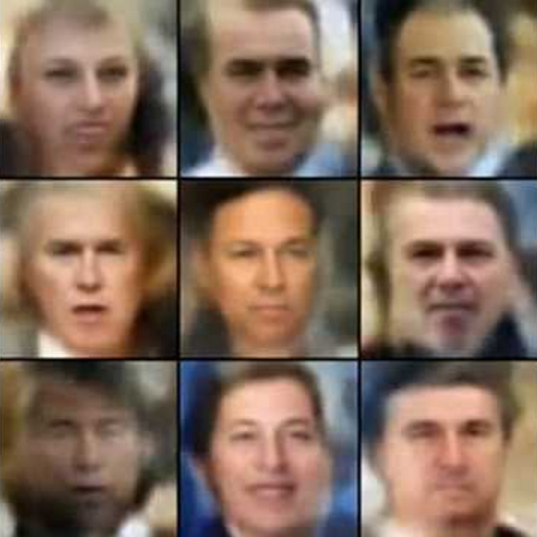
\includegraphics[width = 4in]{../images/VariationalFaces}}
\centerline{[Alec Radford]}


\slide{Summary: Rate-Distortion}

RDA: $y$ continuous, $\tilde{z}$ a bit string,

{\color{red}
\begin{eqnarray*}
\Phi^* &  = &  \argmin_\Phi E_{y \sim \pop} \;|\tilde{z}_\Phi(y)| + \lambda \mathrm{Dist}(y,y_\Phi(\tilde{z}_\Phi(y)))
\end{eqnarray*}
}

\vfill
Gaussian RDA: {\color{red} $z = z_\Phi(y) + \sigma_\Phi(y) \odot \epsilon$,\hspace{2em} $\epsilon \sim {\cal N}(0,I)$}

{\color{red}
\begin{eqnarray*}
\Phi^* & = & \argmin_\Phi E_{y \sim \pop}\left(\begin{array}{l}\;\;\; \;KL(p_\Phi(z|y),{\cal N}(0,I)) \\ \\ + \lambda E_{z\sim p_\Phi(z|y)}\; \mathrm{Dist}(y,y_\Phi(z)) \end{array}\right)
\end{eqnarray*}
}

\vfill
Issue: Do we expect compression to yield useful features?

\slide{END}

}
\end{document}


\slide{Gaussian Variational Autoencoder (Gaussian VAE)}

{\huge  $$\Phi^* = \argmin_{\Phi}\;E_{y\sim \pop} \left(\begin{array}{l}\;\;\;\;\;\;KL(p_\Phi(z|y),{\cal N}(0,I)) \\
\;+\; \; {\color{red} \frac{1}{2(\sigma^*(u))^2}} E_{z\sim p_\Phi(z|y)}\;\mathrm{Dist}(y,\;y_\Phi(z))\end{array}\;\right)$$

\begin{eqnarray*}
z[i] & = & z_\Phi(y)[i] + \sigma_\Phi(y)[i]\epsilon\;\;\;\;\epsilon \sim {\cal N}(0,1) \\
p_\Psi(z[i]) & = & {\cal N}(\mu_\Psi[i],\sigma_\Psi[i]) \\
\mathrm{Dist}(y,y') & = & ||y-y'||^2 \\
\\
{\color{red} \sigma^*(u)} & {\color{red} =} & {\color{red} \argmin_\sigma E_{y \sim \pop,z \sim p_\Phi(z|y)}\; \frac{1}{2\sigma^2}\mathrm{Dist}(y,y_\Phi(z)) + d \ln \frac{\sigma}{u}}
\;\mbox{for $y \in \mathbb{R}^d$}
\end{eqnarray*}

\vfill
\centerline{{\color{red} $u$} is the unit of measure for the components of $y$}

